% !TeX root = ../../main.tex
\subsection{多角形の内角と外角}

まずは三角形について考える.

\begin{definitionbox}{\textbf{三角形の内角と外角}}
    \label{def:三角形の内角と外角}
    三角形の3つの辺がつくる三角形の内部にある角のことを \fitblankbf[内角]{} という.
    これに対し, 1つの辺とそれと隣り合う辺の延長がつくる角のことを
    \fitblankbf[外角]{} という.
\end{definitionbox}

また, 三角形の内角と外角に対して次のことがいえる.

\begin{theorembox}{\textbf{三角形の内角と外角の性質}}
    \label{thm:三角形の内角と外角の性質}
    三角形の3つの内角の和は \fitblankbf[180°]{} である.

    三角形の1つの外角は, \fitblankbf[それと隣り合わない2つの]{} 内角の和に等しい.
\end{theorembox}
\vspace{1em}

三角形の内角と外角, それらの性質を図で表すと上のようになる.
\vspace{2em}

\begin{center}
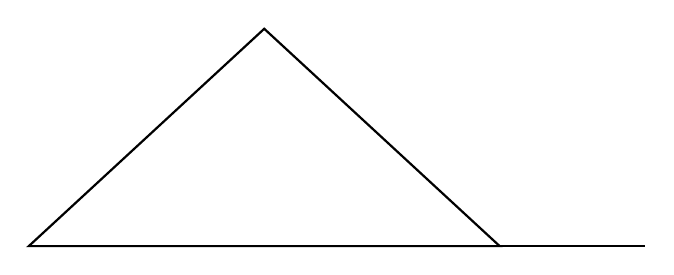
\begin{tikzpicture}[scale=1.15]
    \coordinate (A) at (0,2.4);
    \coordinate (B) at (-2.6,0);
    \coordinate (C) at (2.6,0);
    \coordinate (D) at (4.2,0);
    \draw[thick] (A) -- (B) -- (C) -- cycle;
    \draw[thick] (C) -- (D);
\end{tikzpicture}
\figcap{fig:三角形の内角と外角}{三角形の内角と外角}
\end{center}
\vspace{1em}

Theorem \ref{thm:三角形の内角と外角の性質} より, 図\ref{fig:三角形の内角と外角} において
\fitblankbf[\angle a + \angle b + \angle c = 180°]{}, \fitblankbf[\angle a + \angle b = \angle d]{}

が成り立つ.

\vspace{2em}
次に, 多角形について考える.

\begin{theorembox}{\textbf{多角形の内角の和}}
    \label{thm:多角形の内角の和}
    多角形の内角の和は以下の式で表すことができる.

    \begin{align*}
        \textbf{(n角形の内角の和)} &\bm{=} \fitblankbf[180(n - 2)°]{}
    \end{align*}
\end{theorembox}

\begin{theorembox}{\textbf{多角形の外角の和}}
    \label{thm:多角形の外角の和}
    $n$ 角形の外角の和は \fitblankbf[360°]{} である.
\end{theorembox}

これらの式は, 左辺と右辺をセットで覚え, 使ってもらいたい.


\newpage
